\begin{frame}{Software}
  \Large
  \begin{itemize}
	\item GCFFlasher
	\item deCONZ
    \begin{itemize}
      \Large
      \item Desktop Applikation
      \item Web Applikation
    \end{itemize}
	\item CLI
  \end{itemize}
\end{frame}

\begin{frame}{Software - GCFFlasher}
  \Large
  \begin{itemize}
	\item Firmware für RaspBee
	\item von Dresden Elektronik
	\item zum Flashen und Resetten des RaspBee
  \end{itemize}

  \begin{center}
    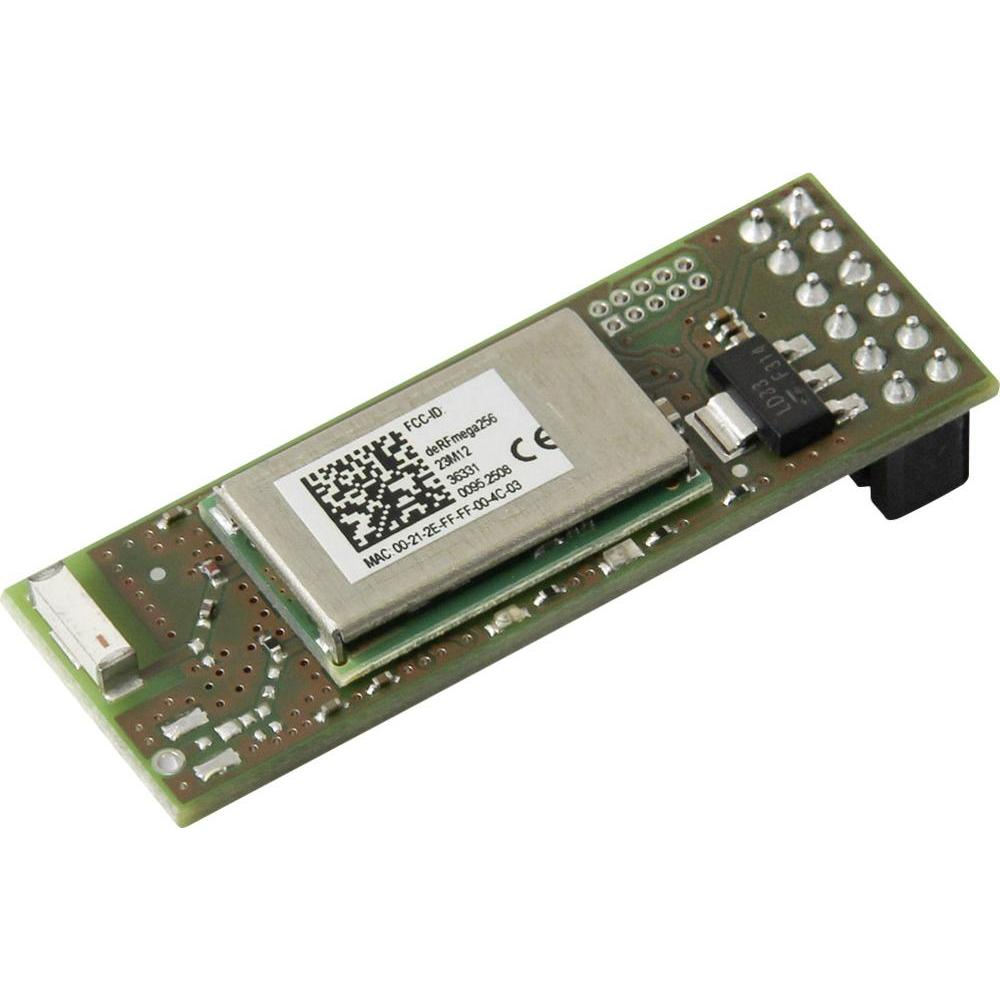
\includegraphics[width=0.5\textwidth]{images/raspbee}
  \end{center}
\end{frame}

\begin{frame}{Software - deCONZ - Desktop Applikation}
  \Large
  Hardwarenahe Steuerung der ZigBee-Nodes

  \begin{center}
    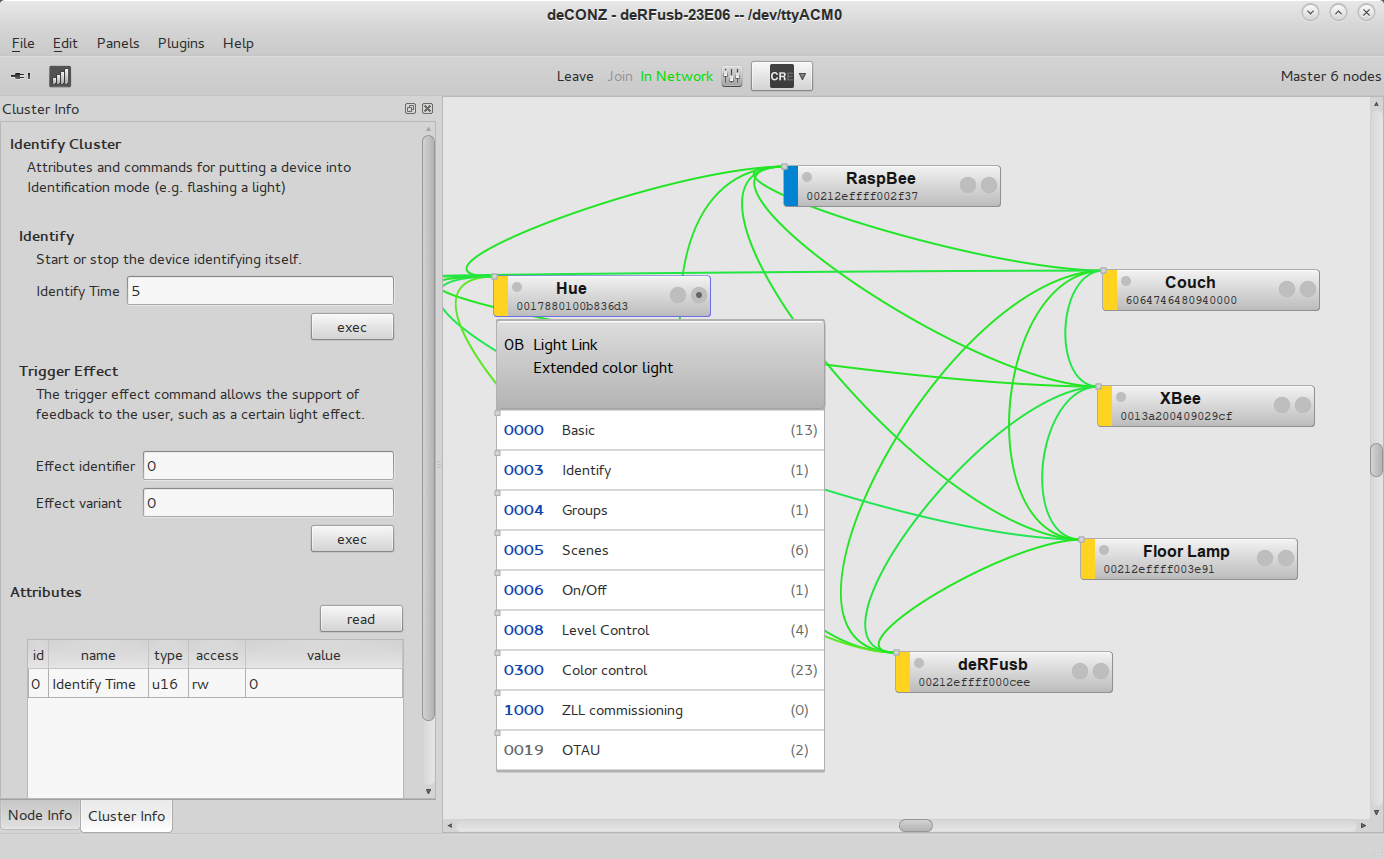
\includegraphics[width=0.8\textwidth]{images/deconz_app}
  \end{center}
\end{frame}

\begin{frame}{Software - deCONZ - Web Applikation}
  \Large
  Erstellung von Gruppen, Szenen über Rest-API

  \begin{center}
    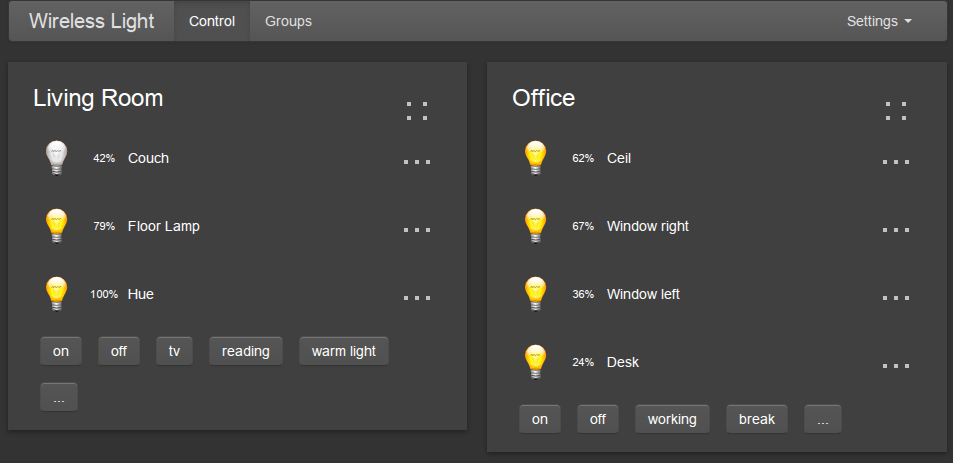
\includegraphics[width=0.8\textwidth]{images/deconz_web}
  \end{center}
\end{frame}

\begin{frame}{Software - CLI - lolo}
  \Large
  \begin{itemize}
    \item Command-Line-Interface
    \item Ruby
    \item clamp
    \item rest-client
    \item nutzt deCONZ Rest-API
  \end{itemize}
\end{frame}